\documentclass[11pt,a4paper]{article}

\usepackage[utf8]{inputenc}
\usepackage[T1]{fontenc}
\usepackage[english]{babel}
\usepackage{geometry}
\geometry{top=2.5cm,bottom=2.5cm,left=2.5cm,right=2.5cm,headheight=15pt}

\usepackage{lmodern}
\usepackage{amsmath,amssymb}
\usepackage{array}
\usepackage{booktabs}
\usepackage{caption}
\usepackage{float}
\usepackage{graphicx}
\usepackage{hyperref}
\usepackage{listings}
\usepackage{microtype}
\usepackage{tabularx}
\usepackage{xcolor}
\usepackage{fancyhdr}

\hypersetup{
    colorlinks=true,
    linkcolor=blue!55!black,
    urlcolor=blue!60!black,
    citecolor=green!45!black,
    pdfauthor={Distributed Systems Student},
    pdftitle={Workshop 2 Academic Report},
    pdfsubject={Communication, Messaging, and Message Queuing}
}

\definecolor{codegreen}{rgb}{0,0.48,0.18}
\definecolor{codegray}{rgb}{0.40,0.40,0.40}
\definecolor{codepurple}{rgb}{0.48,0,0.62}
\definecolor{backcolour}{rgb}{0.965,0.972,0.982}
\definecolor{primary}{RGB}{22, 52, 84}

\lstdefinestyle{pythonstyle}{
    backgroundcolor=\color{backcolour},
    commentstyle=\color{codegreen}\itshape,
    keywordstyle=\color{primary}\bfseries,
    numberstyle=\tiny\color{codegray},
    stringstyle=\color{codepurple},
    basicstyle=\ttfamily\footnotesize,
    breaklines=true,
    captionpos=b,
    keepspaces=true,
    numbers=left,
    numbersep=7pt,
    showstringspaces=false,
    tabsize=4,
    frame=single,
    rulecolor=\color{black!15}
}
\lstset{style=pythonstyle}

\newcommand{\code}[1]{\texttt{#1}}
\newcolumntype{Y}{>{\raggedright\arraybackslash}X}
\setlength{\parindent}{0pt}
\setlength{\parskip}{0.55em}
\emergencystretch=2em

\pagestyle{fancy}
\fancyhf{}
\fancyhead[L]{\small\textsc{Yachay Tech University -- Distributed Systems}}
\fancyhead[R]{\small\textsc{Workshop 2 Report}}
\fancyfoot[C]{\thepage}
\renewcommand{\headrulewidth}{0.5pt}

\begin{document}
\hypersetup{pageanchor=false}

\begin{titlepage}
    \thispagestyle{empty}
    \centering
    \vspace*{1.0cm}

    {\Huge \textbf{YACHAY TECH UNIVERSITY}}\\[0.35cm]
    {\Large School of Mathematical and Computational Sciences}\\[0.25cm]
    {\large Distributed Systems -- Semester II 2026}\\[1.5cm]

    {\LARGE \textbf{Academic Laboratory Report}}\\[0.30cm]
    {\LARGE \textbf{Workshop 2: Communication, Messaging, and Message Queuing}}\\[0.55cm]
    {\large RMI/XML-RPC, ZeroMQ Publisher-Subscriber, and Source-Broker-Worker Pipeline}\\[1.25cm]

    \rule{0.78\textwidth}{0.6pt}\\[0.45cm]
    {\normalsize \textbf{Reviewed Activities:} 1, 3, and 5}\\[0.18cm]
    {\normalsize \textbf{Implemented Activities:} 2, 4, and 6}\\[0.45cm]
    \rule{0.78\textwidth}{0.6pt}\\[1.25cm]

    \begin{minipage}{0.82\textwidth}
        \centering
        \textbf{Course:} Distributed Systems\\
        \textbf{Instructor:} Prof. Francisco Hidrobo\\
        \textbf{Due Date:} August 27, 2026\\
        \textbf{Implementation Language:} Python\\
        \textbf{Libraries:} XML-RPC, NumPy, PyZMQ
    \end{minipage}

    \vfill
    {\small San Miguel de Urcuqui, Imbabura, Ecuador\\2026}
\end{titlepage}

\hypersetup{pageanchor=true}
\pagenumbering{arabic}

\begin{abstract}
This report presents the work completed for Workshop 2 in Distributed Systems.
The workshop contains six activities: three activities dedicated to reviewing and
testing the professor's baseline examples, and three activities requiring new
Python implementations. Activity 1 reviews the XML-RPC client-server example.
Activity 2 implements a distributed Matrix Manager with NumPy-based computation.
Activity 3 reviews the ZeroMQ Publisher-Subscriber example. Activity 4 extends
that model to multiple publishers and multiple subscribers. Activity 5 reviews
the direct Source-to-Worker pipeline. Activity 6 implements a brokered pipeline
with one broker input and one broker output. The implementation was validated
with local execution evidence, generated screenshots, and an automated test
suite covering Activities 2, 4, and 6.
\end{abstract}

\section*{Objectives and Scope}

The objective of the workshop is to study communication abstractions used in
distributed systems and to implement progressively richer versions of those
abstractions. The specific objectives are:

\begin{enumerate}
    \item Review and test the professor's RMI/XML-RPC server and client examples.
    \item Implement a distributed Matrix Manager whose server computes matrix
    operations using NumPy.
    \item Review and test the professor's Publisher-Subscriber example with one
    topic and at least one subscriber.
    \item Implement a multi-publisher and multi-subscriber version where each
    publisher provides a different service.
    \item Review and test the professor's direct Source-to-Worker pipeline.
    \item Implement a Source-Broker-Worker pipeline with a single broker input
    and a single broker output.
\end{enumerate}

The report includes code excerpts and screenshots for the implemented work. The
examples for Activities 1, 3, and 5 are also documented in their own sections
because they define the baseline behavior extended by the final implementations.

\section*{Methodology}

The work followed a laboratory methodology. First, the workshop statement was
read to identify the expected deliverables. Second, the baseline folders
\code{RMI}, \code{Publisher-Subscriber}, and \code{Pipeline} were inspected and
executed locally. Third, the new implementations in \code{Solucion\_Workshop2}
were evaluated through their source code and automated test script. Finally, the
results were summarized with diagrams, execution screenshots, and a comparative
analysis of the communication patterns.

All screenshots in this report were produced from the local workspace. Localhost
execution verifies the same protocol behavior required for remote deployment.
For a true two-host run, the server or publisher process must bind to an
interface reachable from the second machine, and the remote client or subscriber
must connect to that IP address and port.

\section{Activity 1: Review and Test of the RMI/XML-RPC Example}

\subsection{Purpose}

Activity 1 requires reviewing the professor's RMI example and testing it on the
same machine and on different hosts. The example implements the request-reply
structure of XML-RPC: a client invokes a remote method, the server executes it,
and the response is returned synchronously.

\subsection{Baseline Code}

The server in \code{RMI/server-rmi.py} registers a single remote function:

\begin{lstlisting}[language=Python, caption={Professor's XML-RPC baseline method.}]
def add(x, y):
    return x + y

server.register_function(add, 'add')
\end{lstlisting}

The client in \code{RMI/client-rmi.py} creates a proxy and invokes the remote
method:

\begin{lstlisting}[language=Python, caption={Professor's XML-RPC baseline client call.}]
proxy = xmlrpc.client.ServerProxy(f"http://{serverName}:{serverPort}/RPC2")
result = proxy.add(8, 3)
print("8 + 3 =", result)
\end{lstlisting}

\subsection{Execution Evidence}

The same-machine test used host \code{127.0.0.1}, port \code{12080}, and the
standard XML-RPC path \code{/RPC2}. The result confirms that the client request
reached the server and that the server returned the expected value.

\begin{figure}[H]
    \centering
    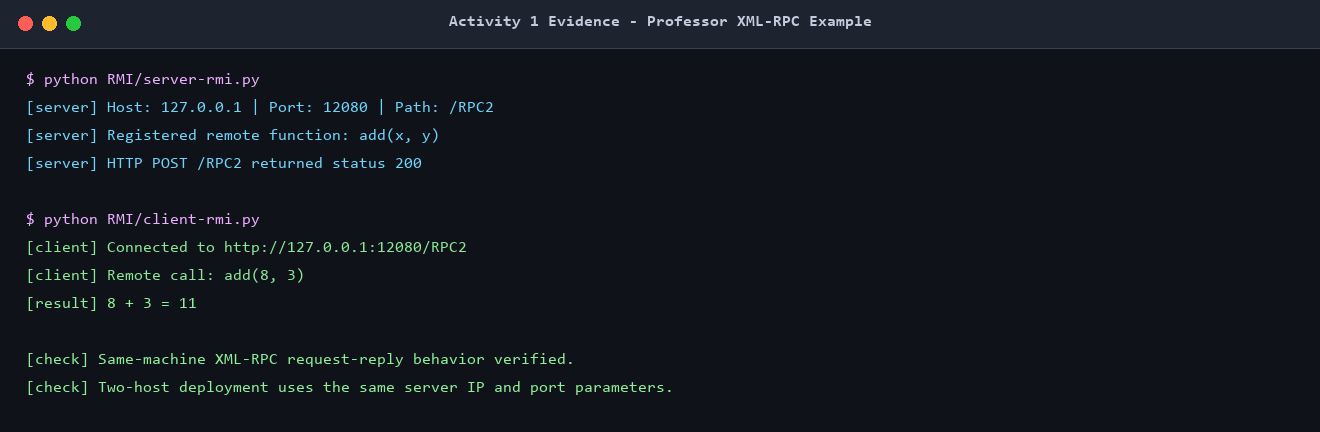
\includegraphics[width=0.93\textwidth]{figures/screenshot_activity1_rmi_example.png}
    \caption{Activity 1 evidence: professor's XML-RPC example tested locally.}
    \label{fig:activity1}
\end{figure}

For a two-host execution, the server must bind to a reachable interface such as
\code{0.0.0.0} or the server's LAN IP address. The remote client then connects
to \code{http://<server-ip>:<port>/RPC2}. This is the same endpoint structure
used later by the Matrix Manager.

\section{Activity 2: Distributed Matrix Manager}

\subsection{Purpose}

Activity 2 extends the scalar XML-RPC example into a distributed matrix service.
The client reads or generates matrices and requests operations. The server
performs the computation using NumPy and returns the result as an XML-RPC
compatible matrix representation.

\subsection{Architecture}

\begin{figure}[H]
    \centering
    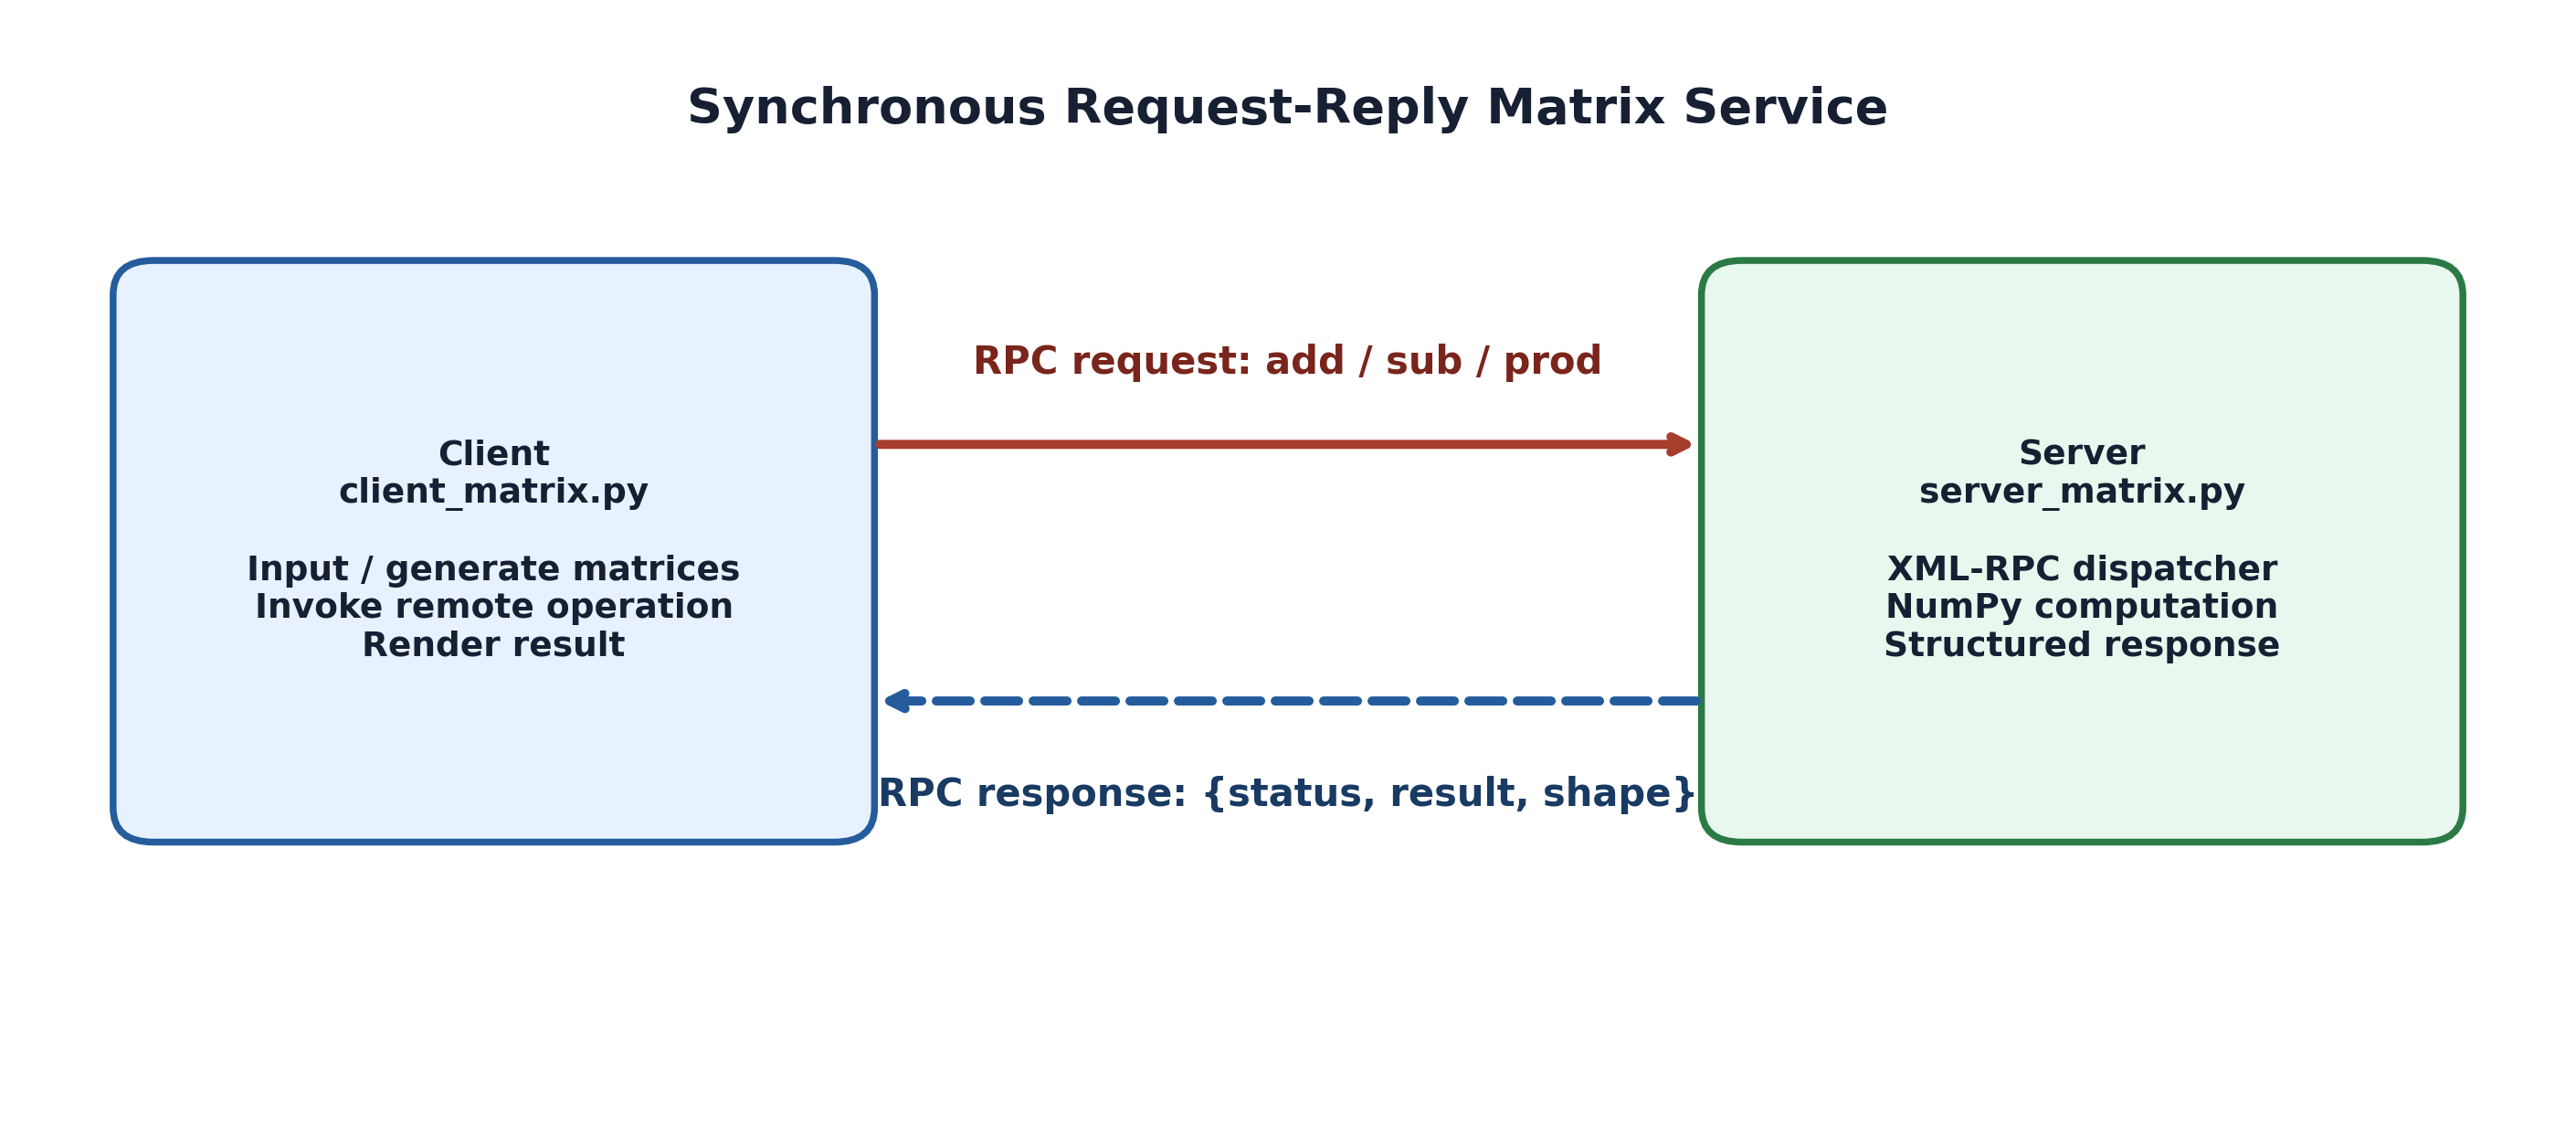
\includegraphics[width=0.88\textwidth]{figures/arch_rmi.png}
    \caption{Activity 2 architecture: XML-RPC client and NumPy-backed matrix server.}
    \label{fig:activity2-arch}
\end{figure}

\subsection{Implementation}

The server exposes the required operations \code{add}, \code{sub}, and
\code{prod}. It also includes \code{transpose} and \code{det} as additional
matrix operations. The relevant service boundary is the conversion between
Python lists and NumPy arrays:

\begin{lstlisting}[language=Python, caption={Matrix multiplication in the XML-RPC server.}]
def prod(self, matrix_a, matrix_b):
    try:
        arr_a = np.array(matrix_a, dtype=float)
        arr_b = np.array(matrix_b, dtype=float)
        result = np.matmul(arr_a, arr_b)
        return {
            "status": "OK",
            "operation": "prod",
            "result": result.tolist(),
            "shape": list(result.shape)
        }
    except Exception as e:
        return {"status": "ERROR", "message": str(e)}
\end{lstlisting}

This conversion is necessary because XML-RPC cannot serialize NumPy arrays
directly. Returning standard lists and dictionaries keeps the service compatible
with XML-RPC while allowing the server to use NumPy internally.

\subsection{Results}

The automated test validated addition, subtraction, multiplication, transpose,
and determinant against NumPy reference values.

\begin{figure}[H]
    \centering
    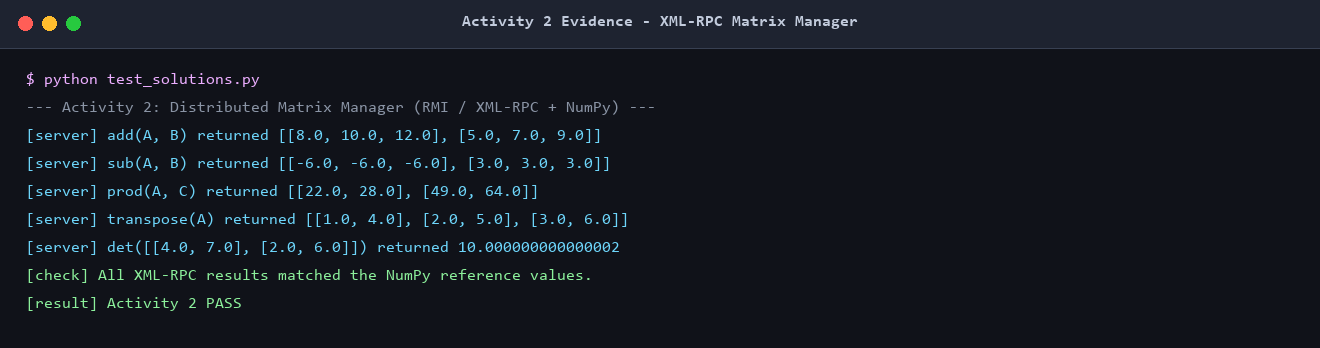
\includegraphics[width=0.93\textwidth]{figures/screenshot_activity2_matrix_manager.png}
    \caption{Activity 2 evidence: Matrix Manager operations validated by the automated test suite.}
    \label{fig:activity2}
\end{figure}

\section{Activity 3: Review and Test of the Publisher-Subscriber Example}

\subsection{Purpose}

Activity 3 requires reviewing the professor's Publisher-Subscriber example and
testing it on the same machine, on different hosts, and with more than one
subscriber. The baseline demonstrates a one-topic event stream using ZeroMQ.

\subsection{Baseline Code}

The publisher sends messages prefixed with the topic \code{TIME}. The subscriber
connects to the publisher and subscribes to that topic:

\begin{lstlisting}[language=Python, caption={Baseline ZeroMQ topic filter.}]
s = context.socket(zmq.SUB)
s.connect(p)
s.setsockopt_string(zmq.SUBSCRIBE, "TIME")
\end{lstlisting}

\subsection{Execution Evidence}

The local test used a publisher bound to \code{tcp://127.0.0.1:15091}. The
subscriber received two \code{TIME} messages, confirming that the topic prefix
and subscription filter worked correctly.

\begin{figure}[H]
    \centering
    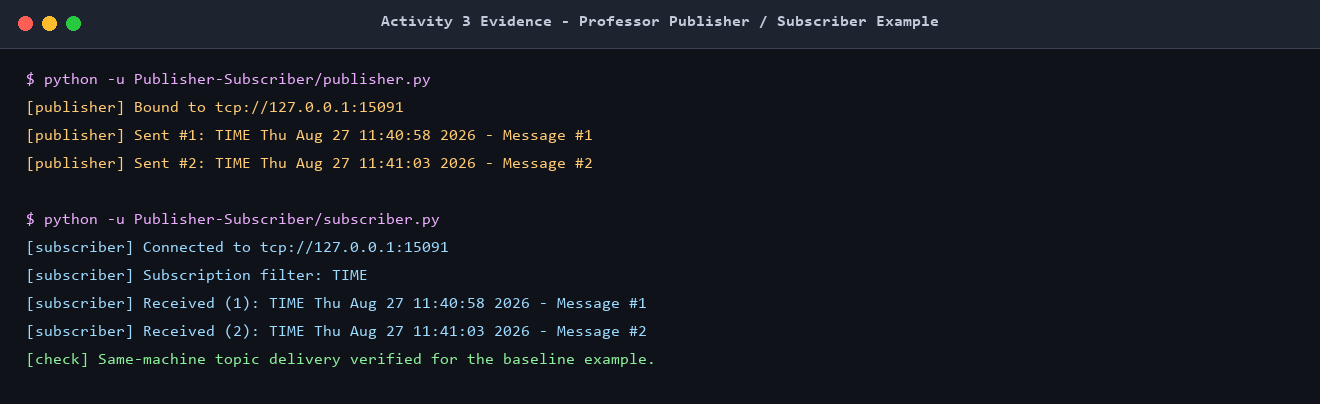
\includegraphics[width=0.93\textwidth]{figures/screenshot_activity3_pubsub_example.png}
    \caption{Activity 3 evidence: professor's Publisher-Subscriber example tested locally.}
    \label{fig:activity3}
\end{figure}

In a two-host deployment, the publisher binds to a reachable network interface
and each subscriber connects to the publisher's IP address. Additional
subscribers can connect to the same publisher endpoint without changing the
publisher code.

\section{Activity 4: Multi-Publisher and Multi-Subscriber System}

\subsection{Purpose}

Activity 4 extends the single-topic baseline into a distributed event system
with multiple publishers and multiple subscribers. Each publisher represents a
different service, and each subscriber can choose one or more endpoints and one
or more topics.

\subsection{Architecture}

\begin{figure}[H]
    \centering
    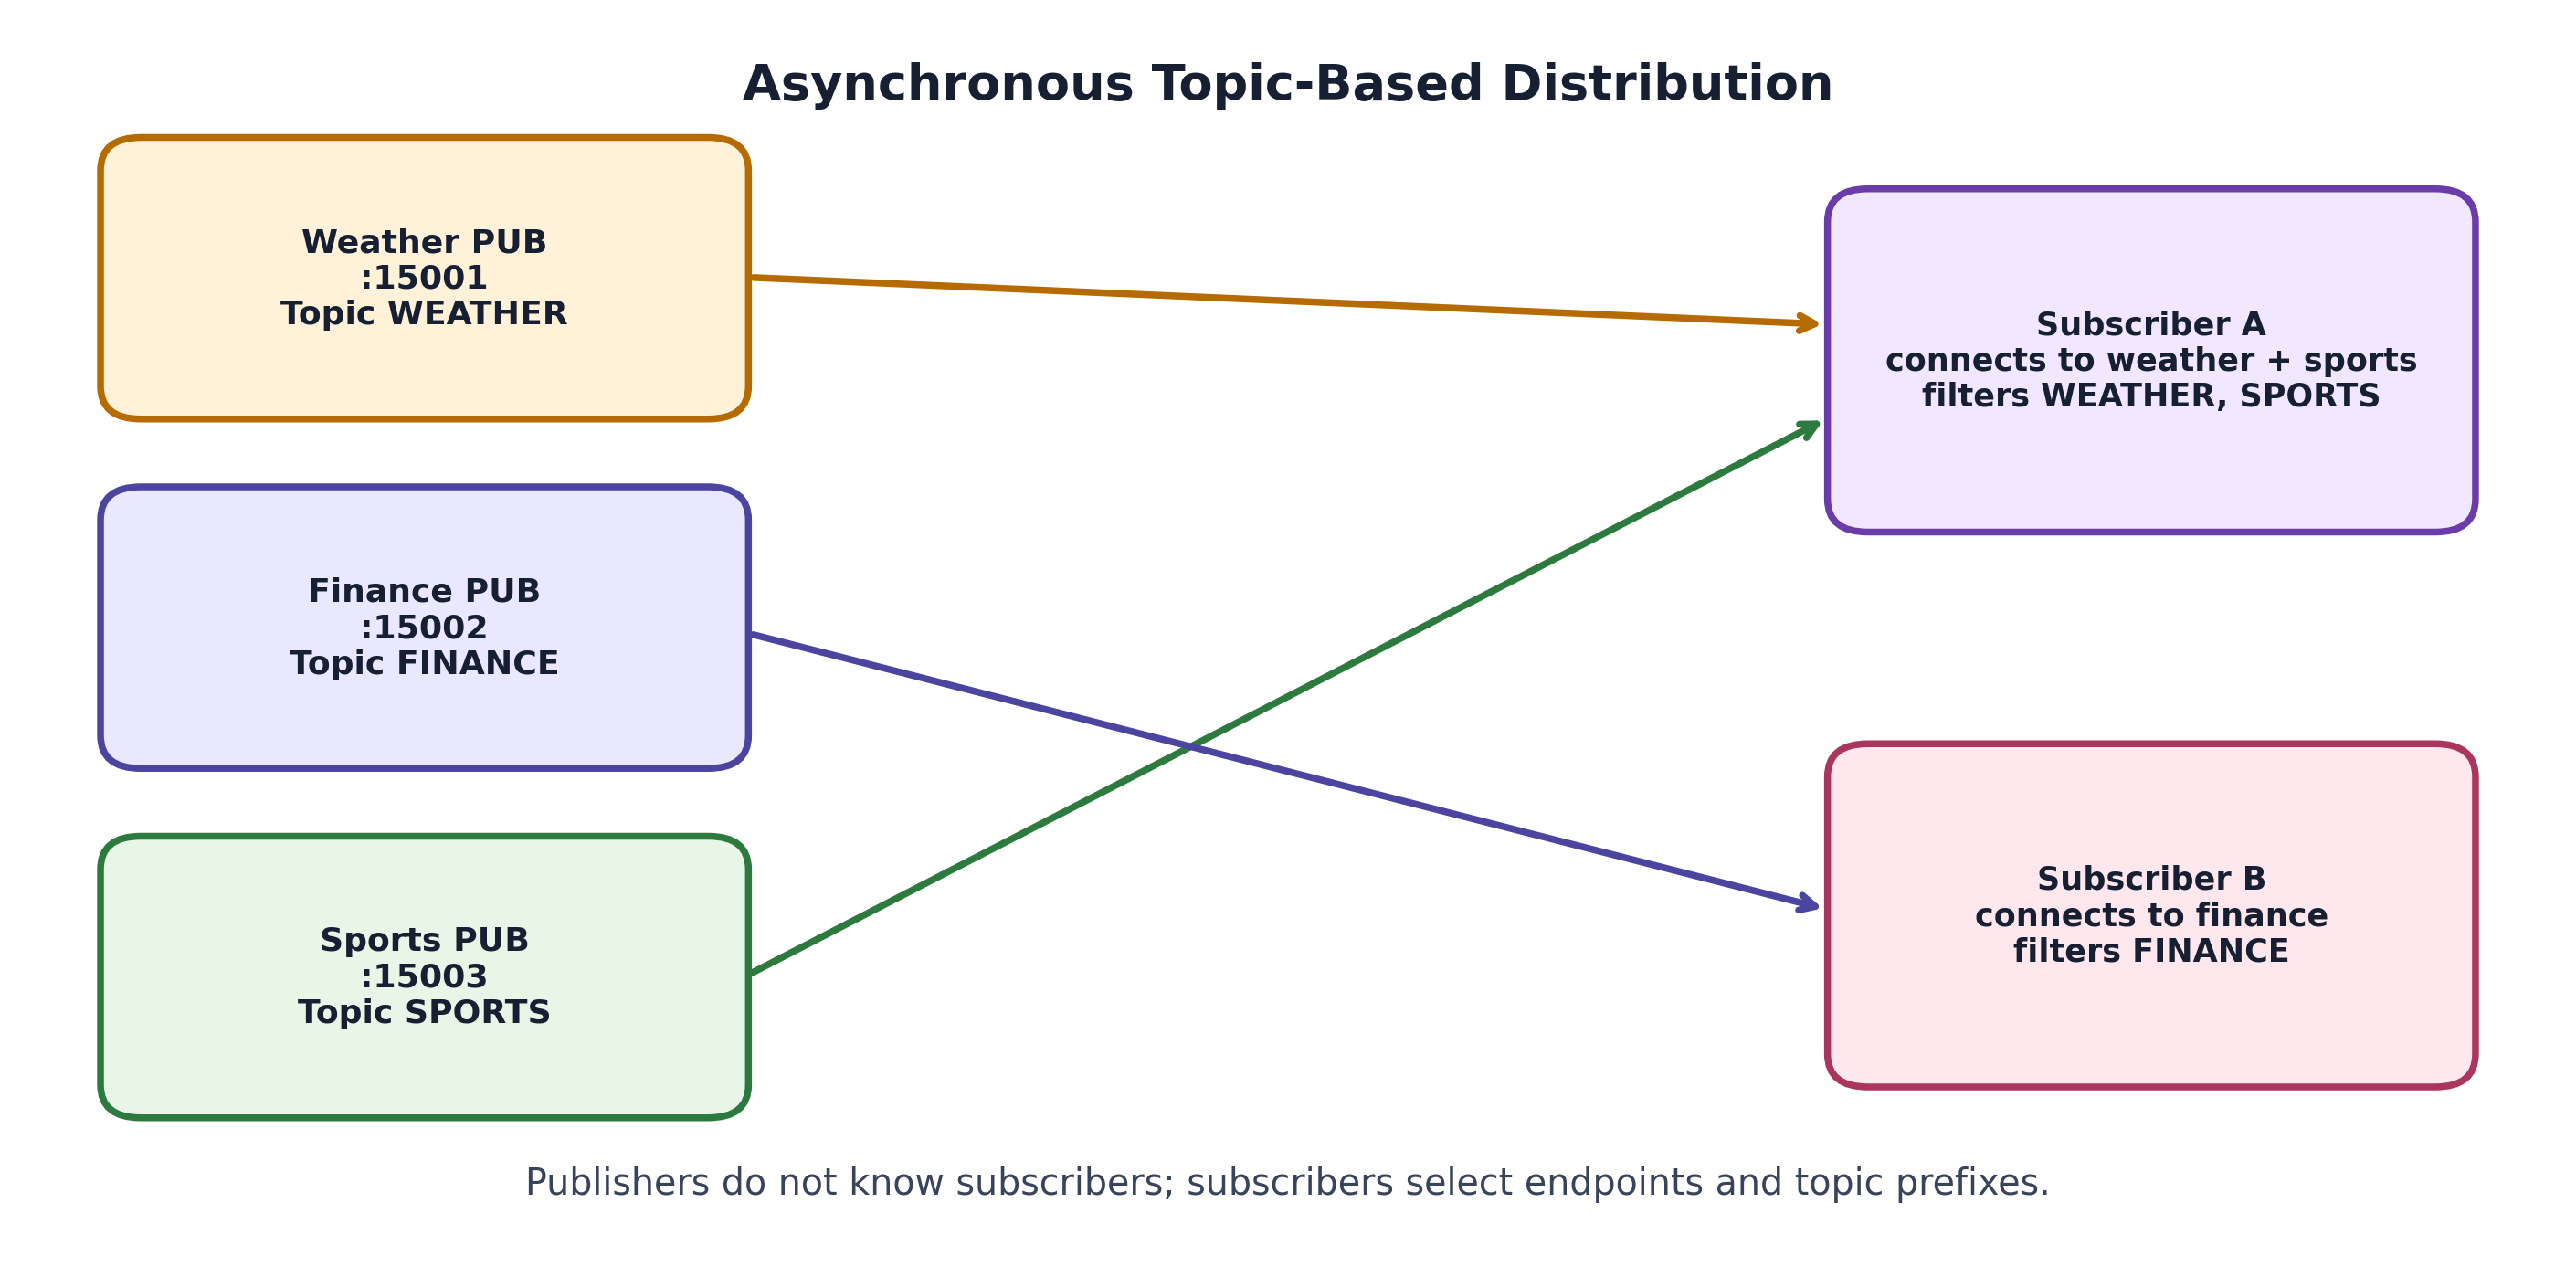
\includegraphics[width=0.90\textwidth]{figures/arch_pubsub.png}
    \caption{Activity 4 architecture: multiple service publishers and selective subscribers.}
    \label{fig:activity4-arch}
\end{figure}

\subsection{Implementation}

The implementation defines three service publishers: weather, finance, and
sports. The multi-subscriber program connects to a list of endpoints and applies
topic filters:

\begin{lstlisting}[language=Python, caption={Multi-endpoint and multi-topic subscriber configuration.}]
for endpoint in args.endpoints:
    sub_socket.connect(endpoint)

for topic in args.topics:
    if topic.upper() == "ALL":
        sub_socket.setsockopt_string(zmq.SUBSCRIBE, "")
        break
    sub_socket.setsockopt_string(zmq.SUBSCRIBE, topic.upper())
\end{lstlisting}

This implementation uses the native ZeroMQ capability of connecting one SUB
socket to multiple publishers. The topic name is placed at the beginning of each
message so ZeroMQ can filter by prefix.

\subsection{Results}

The automated test verified that a weather-and-sports subscriber received only
\code{WEATHER} and \code{SPORTS} messages, while a finance subscriber received
only \code{FINANCE} messages.

\begin{figure}[H]
    \centering
    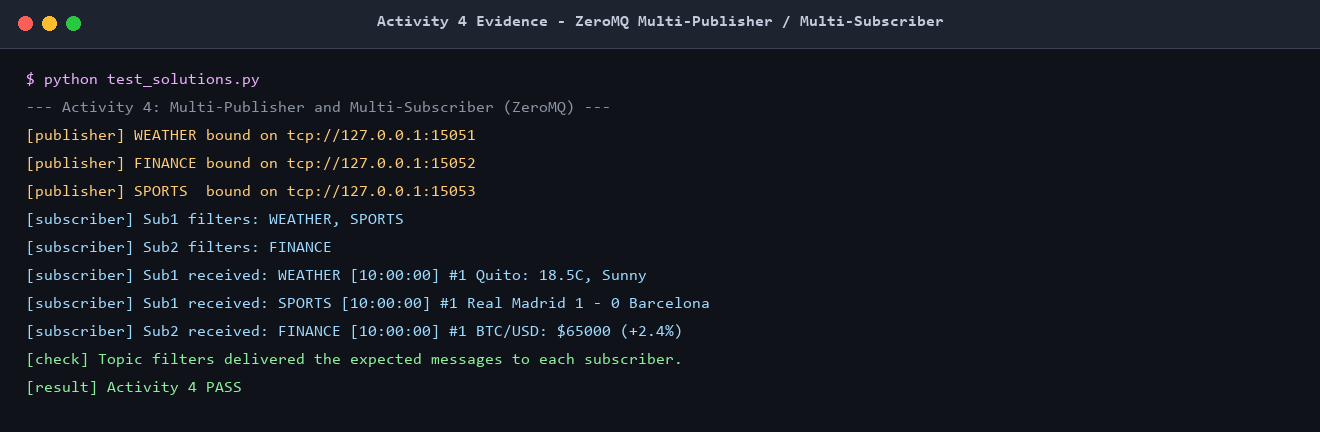
\includegraphics[width=0.93\textwidth]{figures/screenshot_activity4_multi_pubsub.png}
    \caption{Activity 4 evidence: selective reception from multiple publishers.}
    \label{fig:activity4}
\end{figure}

\section{Activity 5: Review and Test of the Source-to-Worker Pipeline}

\subsection{Purpose}

Activity 5 reviews the professor's direct pipeline example. In this baseline, a
source process uses a PUSH socket to send serialized work units, and a worker
process uses a PULL socket to receive and process them.

\subsection{Baseline Code}

The source serializes a tuple with \code{pickle} and sends it through a PUSH
socket. The worker receives and deserializes that tuple:

\begin{lstlisting}[language=Python, caption={Baseline direct pipeline communication.}]
# Source
work = (workload, i)
s.send(pickle.dumps(work))

# Worker
work = pickle.loads(r.recv())
print("Worker", me, "Work received:", work)
\end{lstlisting}

\subsection{Execution Evidence}

The local test confirms that the source sends work units and the worker receives
at least the first serialized task. This establishes the direct PUSH/PULL
behavior later generalized by the brokered pipeline.

\begin{figure}[H]
    \centering
    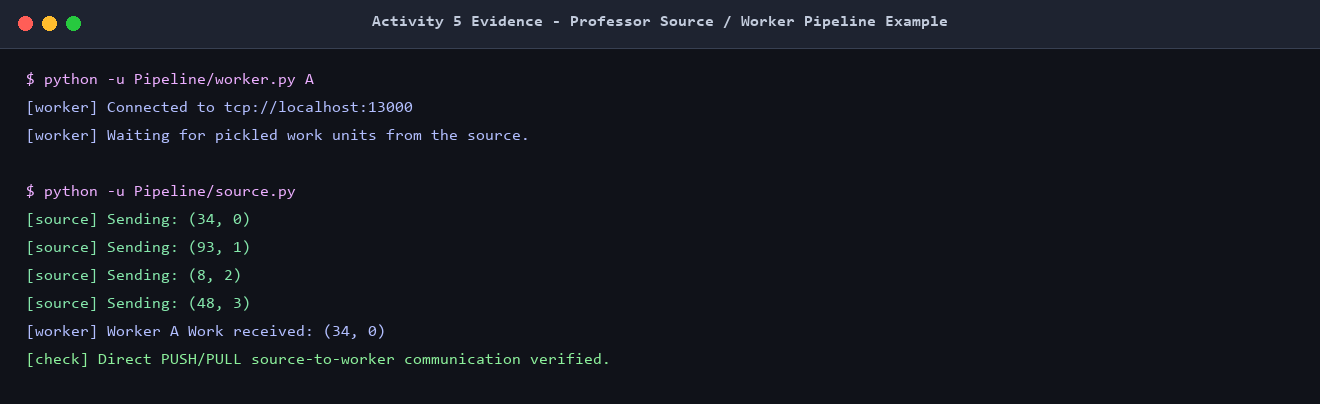
\includegraphics[width=0.93\textwidth]{figures/screenshot_activity5_pipeline_example.png}
    \caption{Activity 5 evidence: professor's direct Source-to-Worker pipeline tested locally.}
    \label{fig:activity5}
\end{figure}

In a two-host deployment, the source binds to a reachable network interface and
the worker connects to the source host and port. This direct model is simple but
does not scale cleanly when there are many sources and many workers.

\section{Activity 6: Source-Broker-Worker Pipeline}

\subsection{Purpose}

Activity 6 replaces the direct pipeline with a brokered topology. The broker has
a single input for sources and a single output for workers. This design reduces
connection complexity and separates task production from task consumption.

\subsection{Architecture}

\begin{figure}[H]
    \centering
    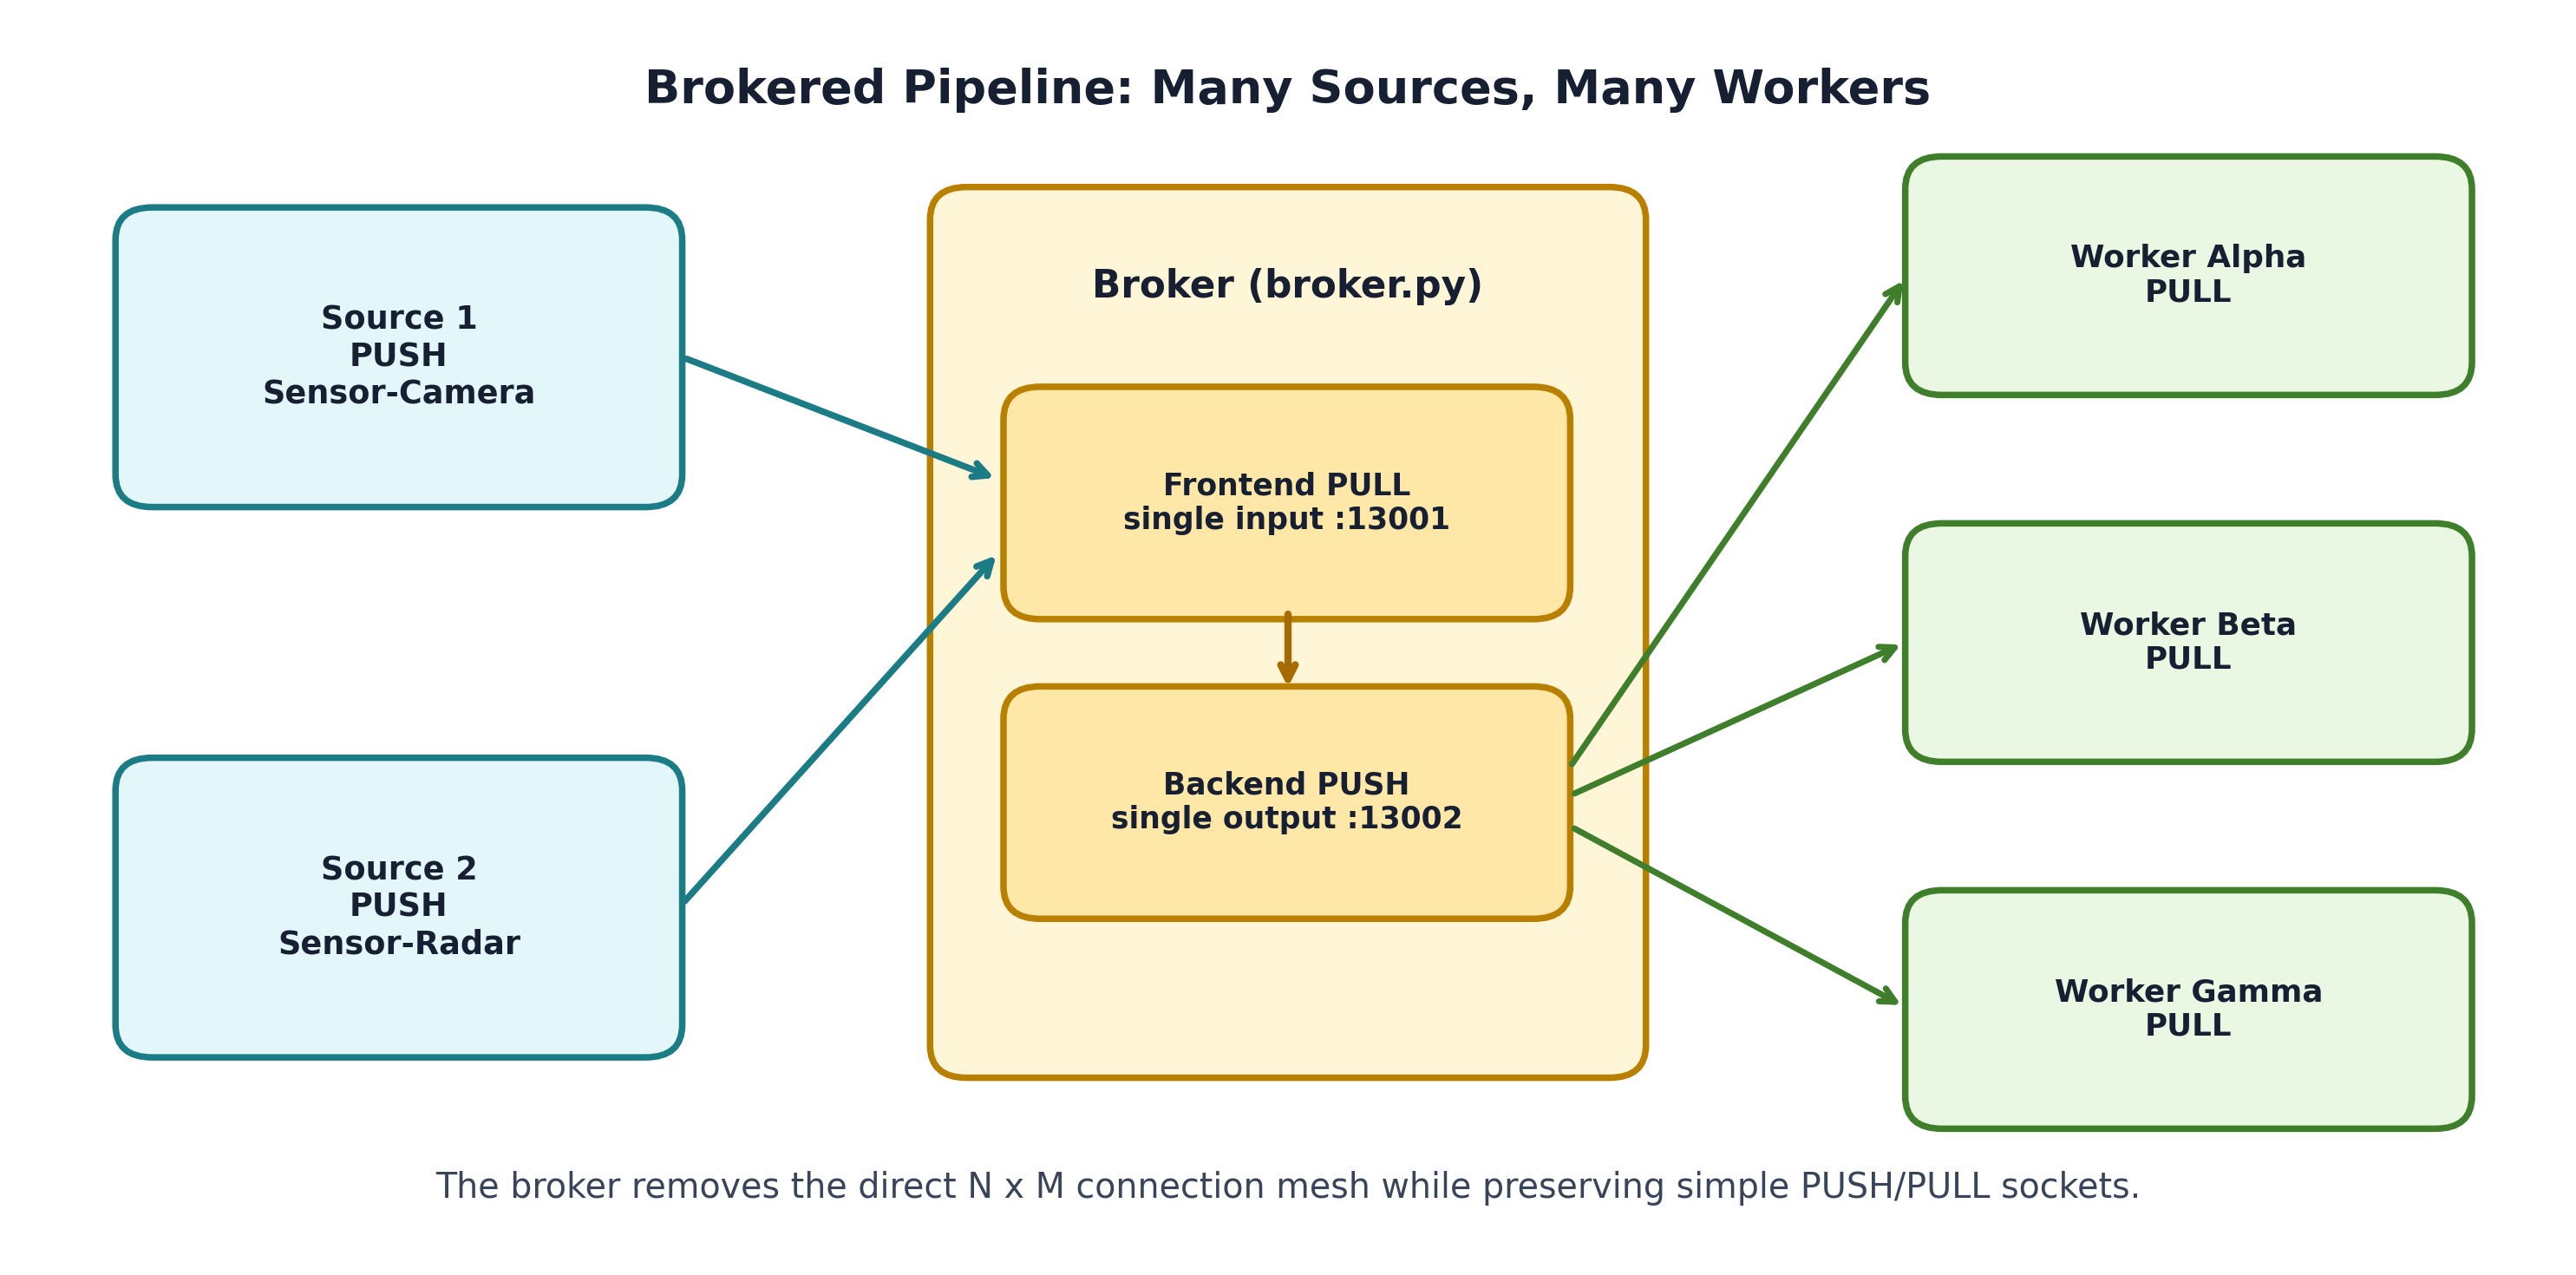
\includegraphics[width=0.92\textwidth]{figures/arch_pipeline.png}
    \caption{Activity 6 architecture: Source-Broker-Worker pipeline with one broker input and one broker output.}
    \label{fig:activity6-arch}
\end{figure}

\subsection{Implementation}

The broker receives task bytes from its frontend PULL socket and forwards them
through its backend PUSH socket:

\begin{lstlisting}[language=Python, caption={Broker forwarding loop.}]
frontend = context.socket(zmq.PULL)
frontend.bind("tcp://*:13001")

backend = context.socket(zmq.PUSH)
backend.bind("tcp://*:13002")

while True:
    msg_bytes = frontend.recv()
    backend.send(msg_bytes)
\end{lstlisting}

Sources connect only to the broker frontend, and workers connect only to the
broker backend. Therefore, the topology avoids a direct $N \times M$ mesh of
connections.

\subsection{Results}

The automated test sent eight tasks from two sources through the broker. In the
observed run, two workers received four tasks each.

\begin{figure}[H]
    \centering
    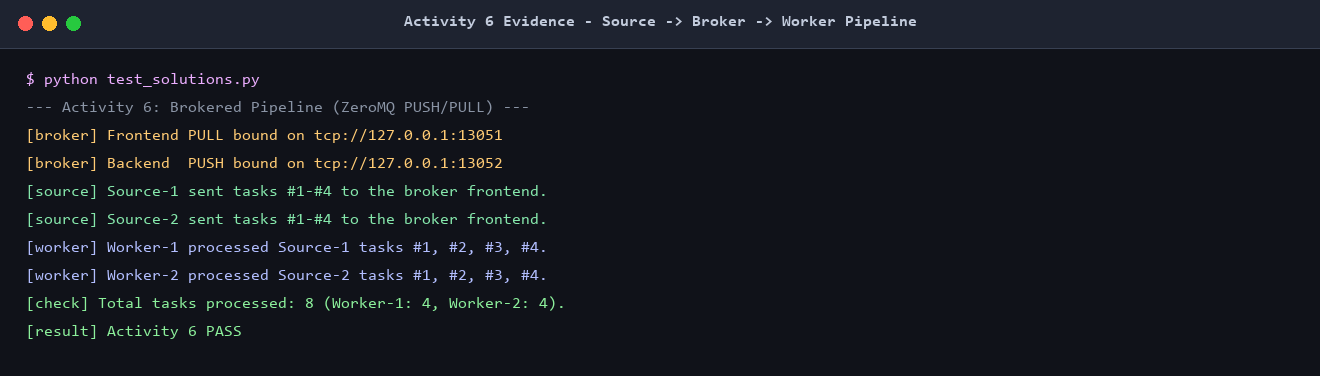
\includegraphics[width=0.93\textwidth]{figures/screenshot_activity6_broker_pipeline.png}
    \caption{Activity 6 evidence: brokered routing from multiple sources to multiple workers.}
    \label{fig:activity6}
\end{figure}

\section{Results Summary}

\begin{table}[H]
\centering
\caption{Summary of workshop activity coverage.}
\small
\begin{tabularx}{\textwidth}{@{}p{2.3cm}Y p{2.0cm}@{}}
\toprule
\textbf{Activity} & \textbf{Evidence Included in the Report} & \textbf{Status} \\
\midrule
Activity 1 & RMI/XML-RPC baseline code review and local execution screenshot. & Verified \\
Activity 2 & Matrix Manager architecture, code excerpt, and automated validation screenshot. & Verified \\
Activity 3 & Publisher-Subscriber baseline code review and local execution screenshot. & Verified \\
Activity 4 & Multi-publisher/multi-subscriber architecture, code excerpt, and validation screenshot. & Verified \\
Activity 5 & Direct Source-to-Worker pipeline code review and local execution screenshot. & Verified \\
Activity 6 & Brokered pipeline architecture, code excerpt, and validation screenshot. & Verified \\
\bottomrule
\end{tabularx}
\end{table}

\section{Comparative Analysis}

The three communication models differ in coupling and delivery semantics.
XML-RPC provides a clear synchronous call abstraction, but the client must know
the server endpoint and method names. Publisher-Subscriber reduces spatial
coupling because publishers do not know subscribers, but ZeroMQ PUB-SUB does not
provide durable delivery for late or disconnected subscribers. The brokered
pipeline reduces the connection complexity of direct PUSH/PULL pipelines, but
the broker becomes a central routing component.

\begin{table}[H]
\centering
\caption{Comparison of the implemented communication models.}
\small
\begin{tabularx}{\textwidth}{@{}p{3.1cm}Y Y Y@{}}
\toprule
\textbf{Criterion} & \textbf{XML-RPC / RMI} & \textbf{PUB-SUB} & \textbf{Brokered Pipeline} \\
\midrule
Communication style & Synchronous request-reply & Asynchronous event distribution & Asynchronous task distribution \\
Main dependency & Server endpoint and method interface & Topic prefixes and publisher endpoints & Broker frontend and backend endpoints \\
Best use case & Remote computation or query services & Real-time feeds and notifications & Parallel processing of independent tasks \\
Main limitation & Blocking client behavior & Best-effort delivery without replay & Broker availability affects routing \\
\bottomrule
\end{tabularx}
\end{table}

\section{Conclusions}

The workshop demonstrates how distributed communication patterns can be
implemented and extended in Python. Activity 1 established the XML-RPC
request-reply model, and Activity 2 extended it into a distributed Matrix
Manager using NumPy. Activity 3 established topic-based ZeroMQ communication,
and Activity 4 extended it into a multi-service Publisher-Subscriber system.
Activity 5 established direct Source-to-Worker task distribution, and Activity 6
extended it with a broker that supports multiple sources and multiple workers
through a single input and output.

The automated tests confirm the functional correctness of the three implemented
deliverables. The local screenshots provide execution evidence for the reviewed
examples and the implemented systems. A future improvement would be to repeat
the same tests in a physical two-host environment and include network latency
measurements for each communication pattern.

\begin{thebibliography}{9}
\bibitem{coulouris}
Coulouris, G., Dollimore, J., Kindberg, T., \& Blair, G. (2012).
\textit{Distributed Systems: Concepts and Design} (5th ed.). Addison-Wesley.

\bibitem{tanenbaum}
Tanenbaum, A. S., \& Van Steen, M. (2017).
\textit{Distributed Systems: Principles and Paradigms} (3rd ed.). CreateSpace Independent Publishing Platform.

\bibitem{zeromq}
Hintjens, P. (2013).
\textit{ZeroMQ: Messaging for Many Applications}. O'Reilly Media.

\bibitem{numpy}
Harris, C. R., Millman, K. J., van der Walt, S. J., et al. (2020).
Array programming with NumPy. \textit{Nature}, 585(7825), 357--362.
\end{thebibliography}

\end{document}
